\documentclass{article}
\usepackage[T1]{fontenc}
\usepackage[utf8]{inputenc}
\usepackage[margin=1in]{geometry}
\usepackage{amsmath}
\usepackage{graphicx}

\newcommand{\HRule}{\rule{\linewidth}{0.5mm}}
\newcommand{\Hrule}{\rule{\linewidth}{0.3mm}}

\title{Lab Report 1}
\author{Yuhuang Chen (804449266), Zeyuan Xu (004255573)}
\date{}


\begin{document}
  \maketitle% prints the title block
  \thispagestyle{empty}

\section{Part 1: 1 Bit ALU}
\subsection{Introduction}
\begin{figure}[h]
  \centering
  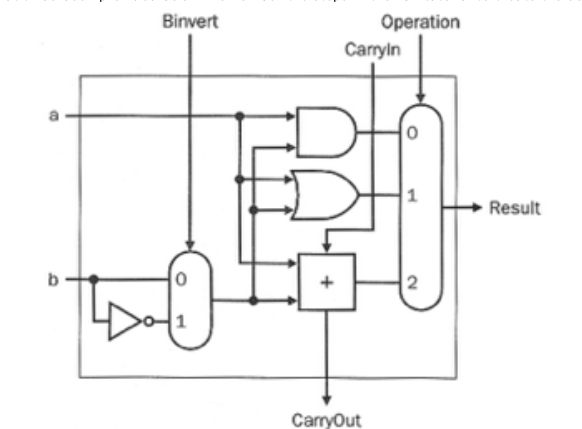
\includegraphics[width=\linewidth]{1-Bit-ALU.png}
  \caption{1-Bit-ALU}
  \label{fig:1-ALU}
\end{figure}
In the first part, we simply need to follow the diagram (figure 1) to implement an 1-bit ALU, which has components as: OR gate, AND gate, NOT gate, 1-bit full adder, 2-1 mux, and 3-1 mux. The 2-1 mux is easily implemented via the logical gate specified in figure 2. The 4-1 mux is simply hooked up in the logic specified in figure 3. 
The schematic diagram is: 
\begin{figure}[!htb]
\minipage{0.5\textwidth}
  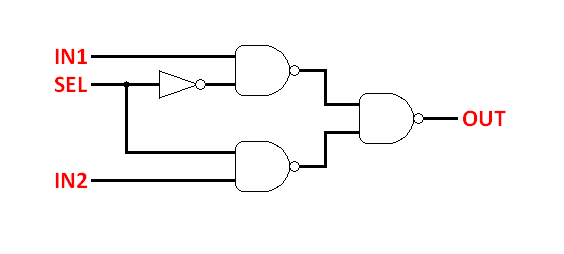
\includegraphics[width=\linewidth]{mux2-1.png}
  \caption{2-1 mux}\label{fig:mux2-1}
\endminipage\hfill
\minipage{0.5\textwidth}
  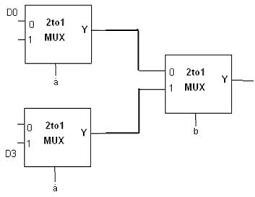
\includegraphics[width=\linewidth]{mux4-1.png}
  \caption{4-1 mux}\label{fig:mux4-1}
\endminipage\hfill
\end{figure}

\subsection{Simulation Result}
The simulation result for the 1-bit ALU is shown in figure 4, in which all operations are tested and verified. 
\begin{figure}[h]
  \centering
  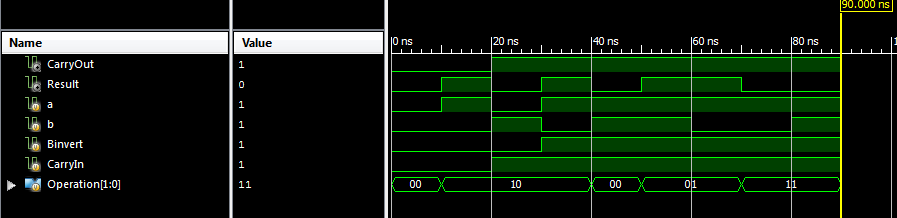
\includegraphics[width=\linewidth]{lab1-1.PNG}
  \caption{1-bit ALU demo}
  \label{fig:1-ALU}
\end{figure}
\subsection{Discussion}
Nothing particular is notieable about the 1-bit ALU. It sets the logic for further implementation of 16 bit ALU, whose structural builds upon it. 

\section{Part 2: 16 Bit ALU}
\subsection{Introduction}
The 16-bit ALU consists consists of operations specified in figure 5. The most complicated part of the ALU design is to design the 16 bit full adder, which should also contain overflow detection. The 16-1 mux is built upon by 4-1 mux, and the logic is depicted in figure 6. The 16-1 mux is shown in figure 7. The adder is implemented as a ripple adder. When buiding the 16-bit adder, we first build 4-bit adder from 1-bit adders, then using the same method to construct the 16-bit adder from the 4-bit adders. The logic can be depicted in figure 8. 
\begin{figure}[h]
  \centering
  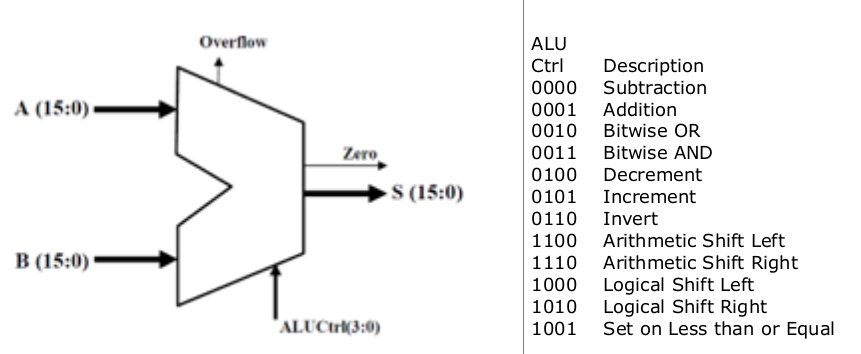
\includegraphics[width=\linewidth]{16-alu.png}
  \caption{16-bit ALU}
  \label{fig:16-ALU}
\end{figure}


\begin{figure}[!htb]
\minipage{0.33\textwidth}
  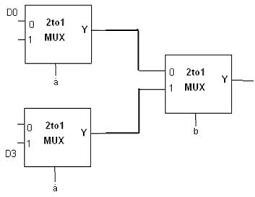
\includegraphics[width=\linewidth]{mux4-1.png}
  \caption{4-1 mux}\label{fig:mux4-1}
\endminipage\hfill
\minipage{0.33\textwidth}
  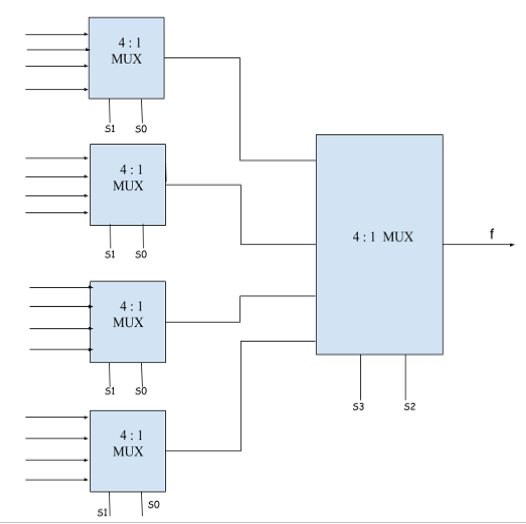
\includegraphics[width=\linewidth]{mux16-1.png}
  \caption{16-1 mux}\label{fig:mux16-1}
\endminipage\hfill
\minipage{0.33\textwidth}
  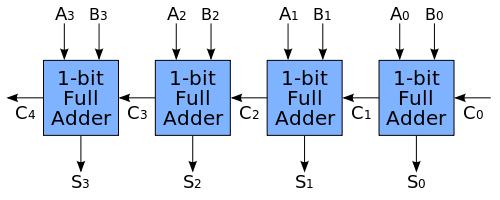
\includegraphics[width=\linewidth]{4-adder.png}
  \caption{4 bit adder}\label{fig:4-adder}
\endminipage\hfill
\end{figure}


\subsection{Simulation Result}

There are 12 operations, so we have in total 12 simulation results, each for one operation.\\
\\
\textbf{1. Subtraction}\\
\begin{figure}[!htb]
  \centering
  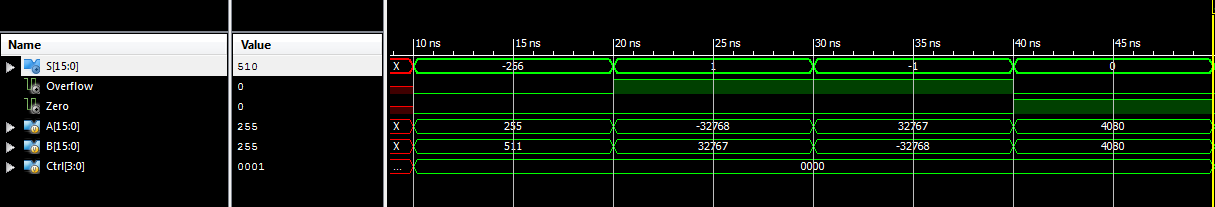
\includegraphics[width=\linewidth]{0000.PNG}
  \caption{subtraction case}
  \label{fig:sub}
\end{figure}
Subtraction's simulation result is shown in the figure 9: the first test case and the fourth test cases do not have overflow, whereas the second and the third test cases, subtracting the largest positive number from the smallest negative number and subtracting the smallest negative number from the largest positive number, all trigger overflow, and the overflow bit is set to high in our simulation. 
\\
\\
\textbf{2. Addition}
\begin{figure}[!htb]
  \centering
  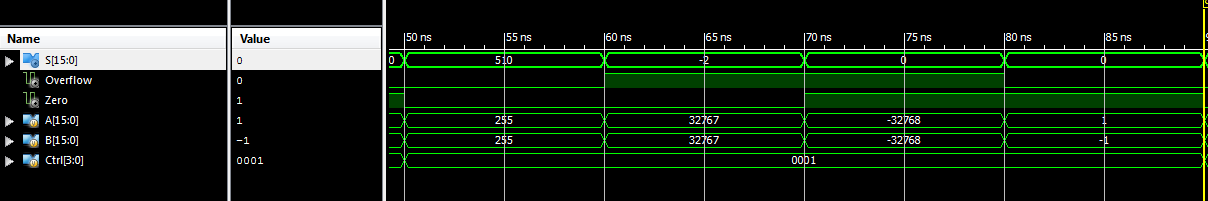
\includegraphics[width=\linewidth]{0001.PNG}
  \caption{addition case}
  \label{fig:add}
\end{figure}

Addition's simulation result is shown in the figure 10: the first test case and the fourth test case do not have overflow, whereas the second and the third test cases, adding the largest positive number with itself and adding the smallest negative number with itself, all trigger overflow, and the overflow bit is set to high in our simulation. 
\\
\textbf{3. Bitwise OR}\\
\begin{figure}[!htb]
  \centering
  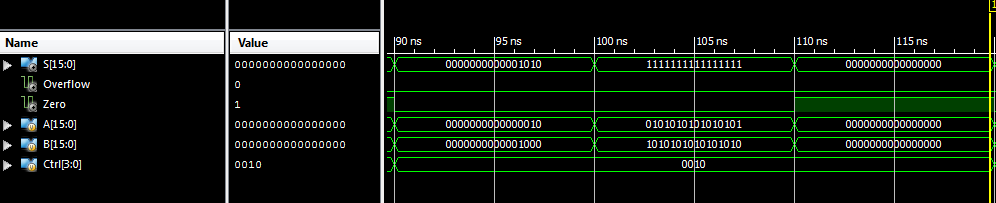
\includegraphics[width=\linewidth]{0010.PNG}
  \caption{bitwise OR case}
  \label{fig:or}
\end{figure}
The bitwise OR's result is in figure 11. In this case, no overflow occurs. \\

\textbf{4. Bitwise AND}\\
\begin{figure}[!htb]
  \centering
  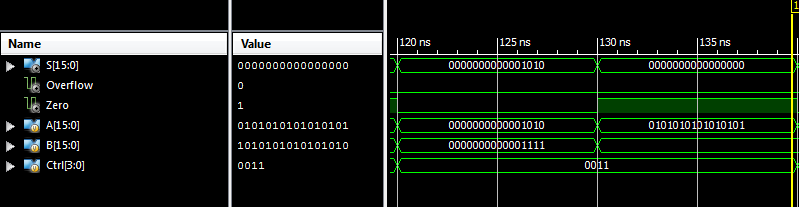
\includegraphics[width=\linewidth]{0011.PNG}
  \caption{bitwise AND case}
  \label{fig:AND}
\end{figure}
The bitwise AND's result is in figure 12. In this case, no overflow occurs.\\

\textbf{5. Decrement}\\
\begin{figure}[!htb]
  \centering
  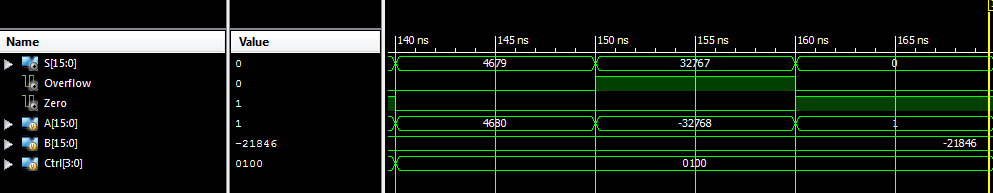
\includegraphics[width=\linewidth]{0100.PNG}
  \caption{Decrement case}
  \label{fig:Decrement}
\end{figure}
The Decrement result is in figure 13. The first and the last cases do not overflow, but the second case, which increments the largest positive number, triggers an overflow and was captured in the simulation. \\

\textbf{6. Increment}\\
\begin{figure}[!htb]
  \centering
  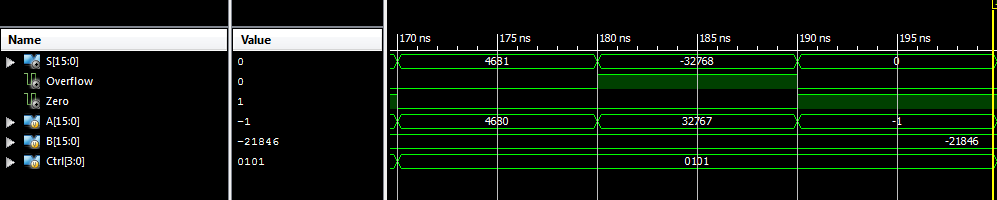
\includegraphics[width=\linewidth]{0101.PNG}
  \caption{Increment case}
  \label{fig:Increment}
\end{figure}
The increment case result is in figure 14. The first and the last cases do not overflow, but the second case, which decrements the smallest negative number, triggers an overflow and was captured in the simulation. \\

\textbf{7. Invert}\\
\begin{figure}[!htb]
  \centering
  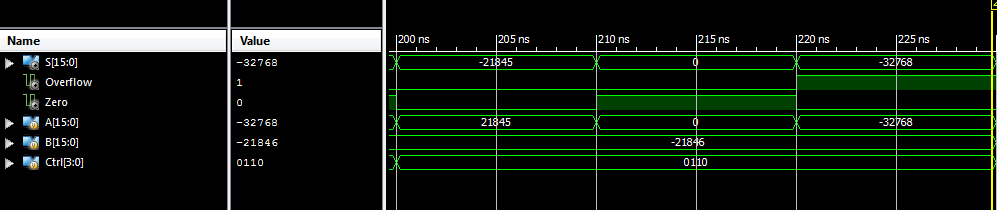
\includegraphics[width=\linewidth]{0110.PNG}
  \caption{Invert case}
  \label{fig:invert}
\end{figure}
The invert case result is in figure 15. The first and the second case do not overflow, but the last case, which inverts the number 16'b1000000000000000, results in an overflow, since the inversion gives the same result back.\\

\textbf{8. Arithmetic Shift Left}\\
\begin{figure}[!htb]
  \centering
  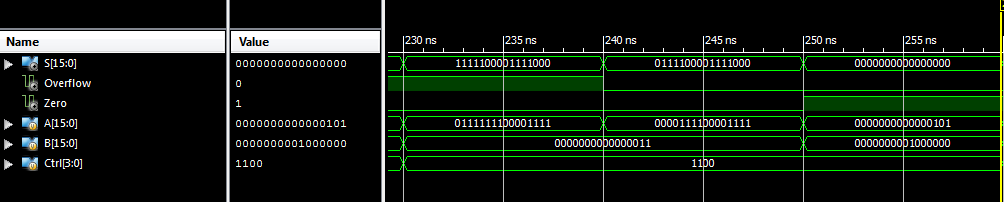
\includegraphics[width=\linewidth]{1100.PNG}
  \caption{Arithmetic Shift Left}
  \label{fig:arith left}
\end{figure}
The result for arithmetic shift left is in figure 16. The first case triggers an overflow. This is because we have an positive number, and left shift should makes another positive number, but a negative number is obtained. \\

\textbf{9. Arithmetic Shift Right}\\
\begin{figure}[!htb]
  \centering
  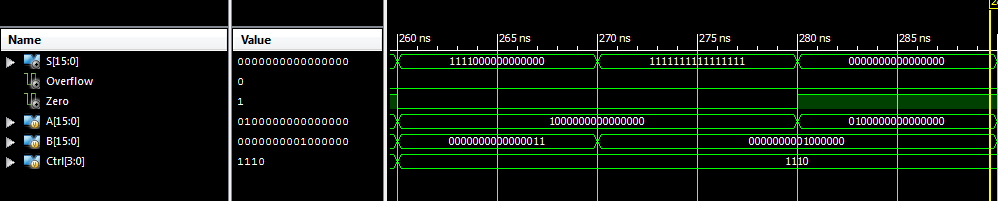
\includegraphics[width=\linewidth]{1110.PNG}
  \caption{Arithmetic Shift Right}
  \label{fig:arith right}
\end{figure}
The result for arithmetic shift right is in figure 17. No overflow occurs for this case. \\

\textbf{10. Logical Shift Left}\\
\begin{figure}[!htb]
  \centering
  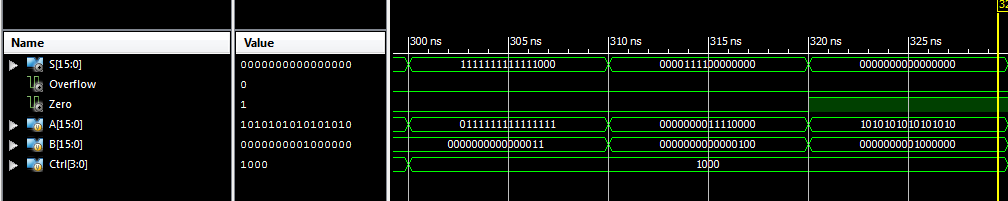
\includegraphics[width=\linewidth]{1000.PNG}
  \caption{Logical Shift Left}
  \label{fig:log left}
\end{figure}
The result for logical shift left is in figure 18. Since it is a logical shift, there is no overflow. \\

\textbf{11. Logical shift Right}\\
\begin{figure}[!htb]
  \centering
  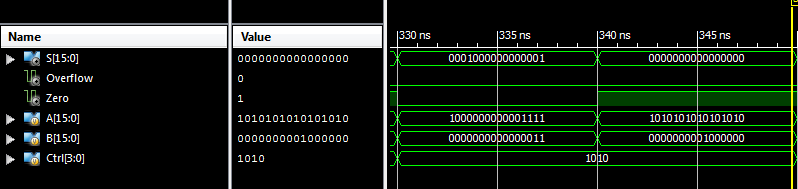
\includegraphics[width=\linewidth]{1010.PNG}
  \caption{Logical Shift Right}
  \label{fig:log right}
\end{figure}
The result for logical shift right is in figure 19. Since it is a logical shift there is no overflow.\\

\textbf{12. Set on Less than or Equal}\\
\begin{figure}[!htb]
  \centering
  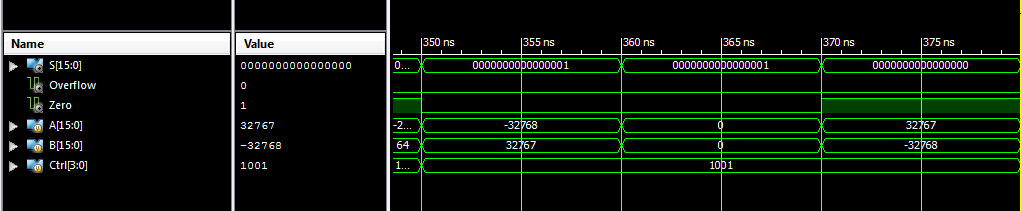
\includegraphics[width=\linewidth]{1001.PNG}
  \caption{slt case}
  \label{fig:slt}
\end{figure}

The result for the set less than or equal case is in figure 20. Even though the subtraction logic might trigger overflow, it should not and is not captured here. 


\subsection{Overflow Detection}
\textbf{Subtraction}: A - B has overflow in two cases: A is positive, B is negative and the result is negative; and A is negative, B is positive and the result is positive. So overflow happens when A and B have different sign and result is the opposite sign as A. We implemented this logic by: 
\begin{verbatim}
assign o0 = (A[15] ^ B[15]) & (A[15] ^ r0[15]);
\end{verbatim}
\vspace{5mm}
\textbf{Addition}: A + B has overflow in two cases: A is positive, B is positive, and the result is negative; and A is negative, B is negative, and the result is positive. So overflow happens when A and b have the same sign and the result is the opposite sign. We implemented this logic by:
\begin{verbatim}
assign o1 = (A[15] ~^ B[15]) & (A[15] ^ r1[15]);
\end{verbatim}
\vspace{5mm}
\textbf{Left Shift}: 
Both arithmetic and logic left shift can trigger overflow: when before and after the operation, the sign of the operand changes, we detect an overflow. We implemented this with the logic: 
\begin{verbatim}
assign o12 = A[15] ^ r12[15];
assign o14 = A[15] ^ r14[15];
\end{verbatim}
\vspace{5mm}
<<<<<<< HEAD
\textbf{Set Less Than}: 
Since the set less than only cares about one bit (either 0 or 1), the code is as follows: 
\begin{verbatim}
assign r9[15:1] = 15'b000000000000000;
	assign r9[0] = (~o9 & ((~r0[15]) | subtract_zero)) | (o9 & (~A[15])); //consider overflow
\end{verbatim}
=======
\textbf{Set Less Than}: The set less than 



\section{Part 3: Register File }
\subsection{Introduction}
The register file is built from 32 16-bit registers, two read ports, and a single write port. The register file should be able to support two concurrent read operations and one write operation. In addition, the register file has a clock and a reset pin. When reset is triggered, all of the registers are set to zeros. The implementation is carried out using behavior verilog. 
\subsection{Simulation Result}



\section{Part 4: Questions and Answers}
Q1: What is the difference between structural and behavior verilog? Please provice an exmaple of a structural and behavior implementation of a multiplexer. \\
A: Behavior verilog refers to verilog design that simulates the behavior of digital circuits using higher order logic and modules, such as using always and assign. Structural verilog refers to verilog design that builds the components from scratch by using logical gates and lower level blocks.  \\
Behavior verilog: 
\begin{verbatim}
module  mux_behavior(din_0, din_1, sel, mux_out); 
input din_0, din_1, sel;
output mux_out;
wire mux_out;
assign mux_out = (sel)? din_1 : din_0;
endmodule
\end{verbatim}
Structural Verilog:
\begin{verbatim}
module mux(f, a, b, sel);
output f;
input a, b, sel;

and g1(f1, a, nsel);
	g2(f2, b, sel); 
or  g3(f, f1, f2);
not g4(nsel, sel); 
endmodule 
\end{verbatim}

Q2: What is the difference between an asynchronous and synchronous multiplexer? Please provide a brief explanation on how you could implement both using behavior verilog. \\
\vspace{5mm}

Q3: What is the difference between an arithmetic and logical shifter?\\
A: Arithmetic shift preserves the sign bit and functions logically equivalent as binary arithmetic; logical shift simply shift out digits and pad with zeros.\\

Q4: Assuming that you did not use Behavior verilog to implement an arithmetic shifter, how could you design one from scratch? Please include a simple diagram.\\
The diagram is simply the following: 
\begin{figure}[!htb]
  \centering
  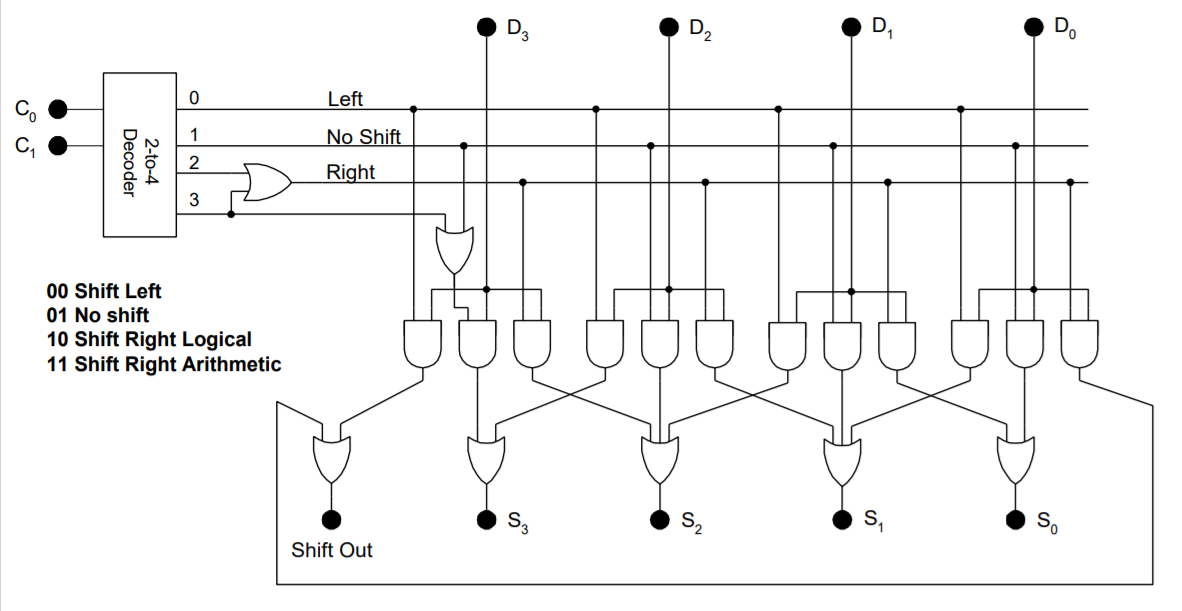
\includegraphics[width=\linewidth]{arithmetic_shift.png}
  \caption{arithemtic}
  \label{fig:arithemtic shift}
\end{figure}












>>>>>>> 91bac4e9b130fddc5a8699f009f85c11f4c48ce5



\section{Part 3: Register File }
\subsection{Introduction}
The register file is depicted in figure 21: \\
\begin{figure}[!htb]
  \centering
  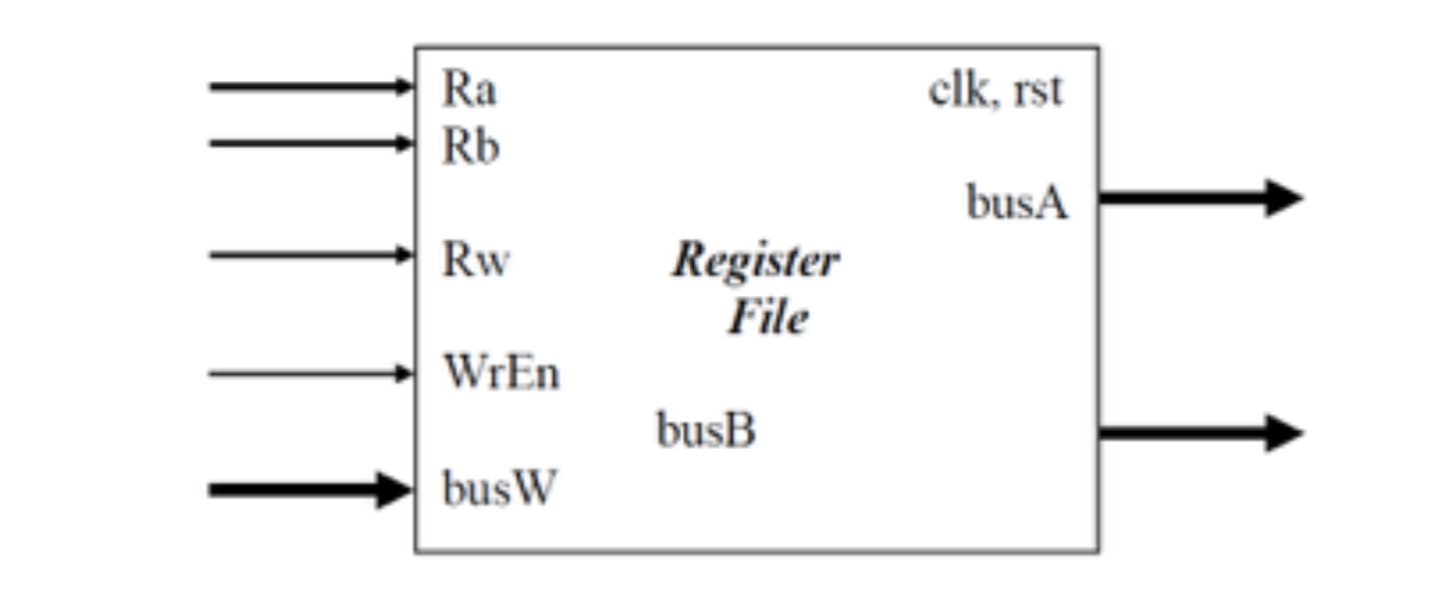
\includegraphics[width=\linewidth]{reg.png}
  \caption{register}
  \label{fig:reg}
\end{figure}
The register file has two 5 inputs and 2 outputs: bus signals are 16 bits and Ra, Rb, Rw are 5 bits. It also has reset and clock pins. \\
The register is implemented in behavior Verilog. 
\subsection{Simulation Result}
The simulation result is shown in figure 22. 
\begin{figure}[!htb]
  \centering
  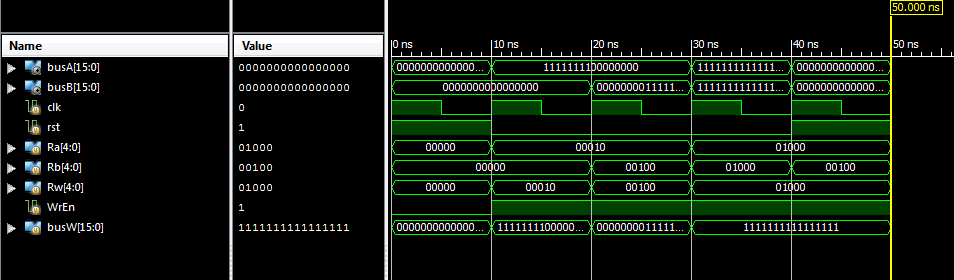
\includegraphics[width=\linewidth]{lab1-3.PNG}
  \caption{register result}
  \label{fig:reg_res}
\end{figure}
The result behaves correctly.
\subsection{Discussion}
Not many problems are encountered in the register implementation. 

\section{Part 4: Questions and Answers}
1. What is the difference between structural and behavioral Verilog? Please provide an example of a structural and behavioral implementation of a multiplexer.\\
A: behavior verilog is more high level and could use always block and assign operations; structural verilog focuses more on the individual building blocks of a module, such as building a complex module using gates.  \textbf{Multiplexer structural implementation}: 
\begin{verbatim}
module mux7( select, d, q );

input[1:0] select;
input[3:0] d;
output     q;

<<<<<<< HEAD
wire       q, q1, q2, q3, q4, NOTselect0, NOTselect1;
wire[1:0]  select;
wire[3:0]  d;

not n1( NOTselect0, select[0] );
not n2( NOTselect1, select[1] );

and a1( q1, NOTselect0, NOTselect1, d[0]  );
and a2( q2,  select[0], NOTselect1, d[1]  );
and a3( q3, NOTselect0,  select[1], d[2]  );
and a4( q4,  select[0],  select[1], d[3]  );
=======


>>>>>>> 91bac4e9b130fddc5a8699f009f85c11f4c48ce5

or o1( q, q1, q2, q3, q4 );

endmodule
\end{verbatim}

\textbf{Multiplexer behavior implementation}: 
\begin{verbatim}
module mux1( select, d, q );

input[1:0] select;
input[3:0] d;
output     q;

wire      q;
wire[1:0] select;
wire[3:0] d;

assign q = d[select];

endmodule
\end{verbatim}

\vspace{10mm}
2. What is the difference between an asynchronous and synchronous Multiplexer? Please provide a brief explanation on how you could implement both using behavioral Verilog.\\
\vspace{10mm}

3. What is the difference between an arithmetic and logical shifter? \\
A: arithmetic shifter and logical shifter behaves the same when doing left shift, but arithmetic shift right replicates the sign bit, while logical shift only keeps padding zeros for the shifted bits. 
\vspace{10mm}

4. Assuming that you did NOT use Behavioral Verilog to implement an arithmetic shifter, how could you design one from scratch? Please include a simple diagram.\\
A: it can be implemented using gates, as shown in figure 23: this shifter shifts a 4-bit value, and similar logic can be applied to an n-bit shifter as well. 
\begin{figure}[!htb]
  \centering
  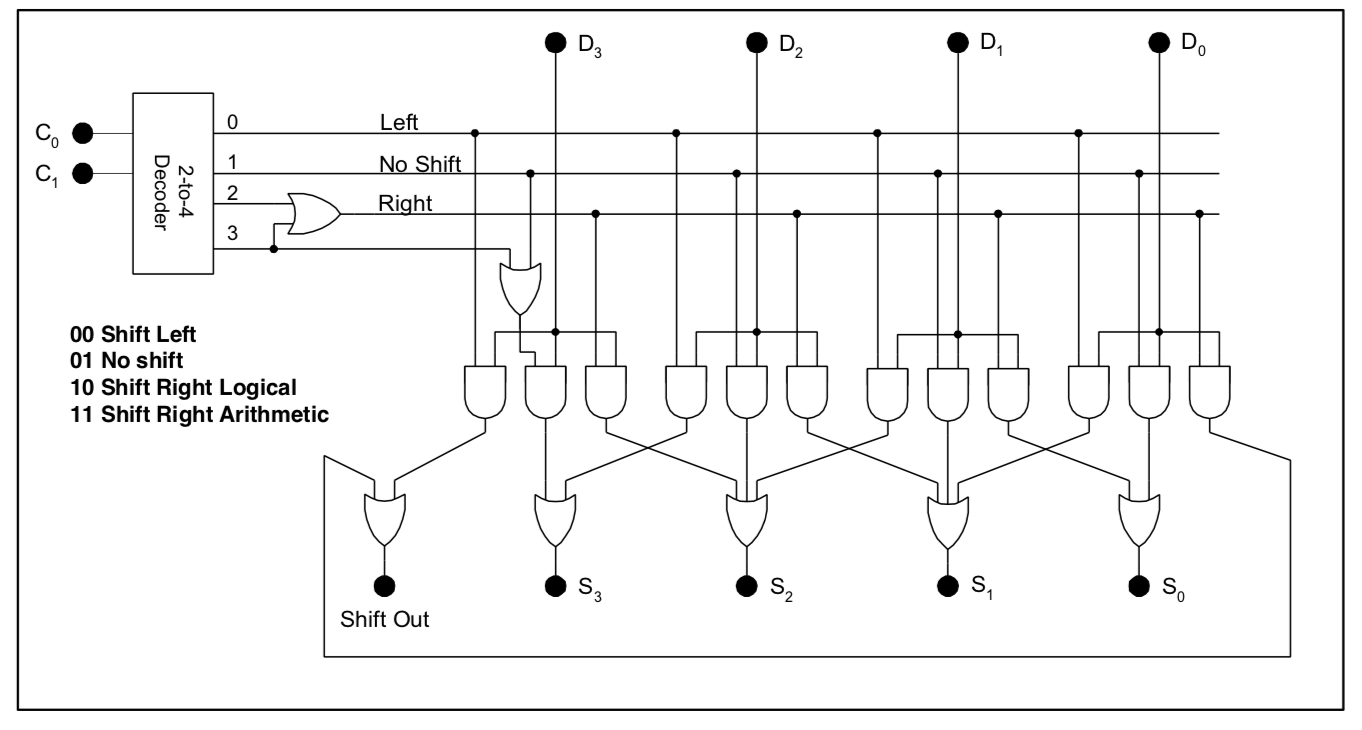
\includegraphics[width=\linewidth]{shifter.png}
  \caption{shifter}
  \label{fig:shift}
\end{figure}



\end{document}